\documentclass[tikz,border=2pt]{standalone}
\usepackage{amsmath,amssymb}
\usepackage{tikz}
\usetikzlibrary{arrows.meta}

\begin{document}
% |z| is the length of the arrow from 0 to z = a + bi: the hypotenuse of a right triangle
% with legs a and b.
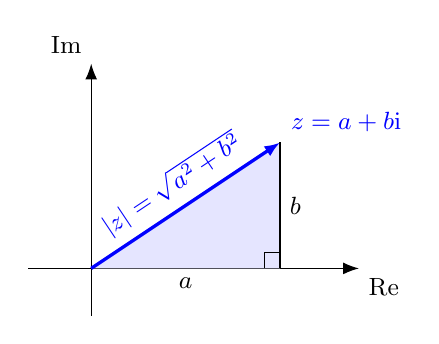
\begin{tikzpicture}[every node/.style={font=\small}, >={Latex[length=2mm]}]
	\draw[->] (-0.8,0) -- (3.4,0) node[below right] {$\mathrm{Re}$};
	\draw[->] (0,-0.6) -- (0,2.6) node[above left] {$\mathrm{Im}$};
	\fill[blue!10] (0,0) -- (2.4,0) -- (2.4,1.6) -- cycle;
	\draw[->, blue, very thick] (0,0) -- (2.4,1.6) node[midway, above, sloped] {$|z|=\sqrt{a^2+b^2}$} node[above right] {$z=a+b\mathrm{i}$};
	\draw[thick] (2.4,0) -- (2.4,1.6);
	\draw (2.2,0) -- (2.2,0.2) -- (2.4,0.2);
	\node[below] at (1.2,0) {$a$};
	\node[right] at (2.4,0.8) {$b$};
\end{tikzpicture}
\end{document}
